\section{Implementação}

Pode-se dividir a implementação em seis partes: segmentação de imagens, seleção de contorno, geração procedural de mapas com biomas, criação de testes para avaliar a geração procedural, análise de casos de pós-processamento e interligação das ferramentas através de uma interface gráfica.

\subsection{Segmentar imagens}

A segmentação de imagem é utilizada para classificar os pixels de uma imagem a partir de padrões reconhecidos por uma inteligência artificial. Isso permite ao usuário selecionar o contorno para gerar o mapa \cite{dp_semantic_segmantation, lapix}.

Para a fotografia urbana, utilizou-se o modelo EfficientPS que, segundo \citeonline{mohan2020efficientps}, é uma solução eficiente para a segmentação panóptica. Utilizou-se também o código disponibilizado no repositório de \citeonline{efficientpsGit}.

Empregou-se um arquivo pré-treinado deste modelo, contendo o aprendizado do conjunto de imagens do \textit{Cityscapes} para segmentação panóptica. A ideia inicial era treinar com pelo menos mais um conjunto de dados, mas surgiram diversos desafios, incluindo a obtenção de autorização para baixar conjuntos de dados específicos, a preparação desses conjuntos para o processo de aprendizado e limitações de capacidade de processamento. Portanto, optou-se por utilizar o próprio modelo salvo, baixado do repositório.

Percebeu-se que o resultado do modelo não foi o esperado, pois objetos da mesma classe, como carros, tinham a mesma cor com uma borda branca, conforme exemplificado na \cref{fig:resultado_inicial}. Assim, tentou-se alterar o código para gerar uma saída com objetos da mesma classe em cores diferentes, conforme ilustrado na \cref{fig:expectativa} no artigo de \citeonline{mohan2020efficientps}, onde cada carro possui uma cor distinta e não há bordas entre os objetos.

\begin{figure}[!ht]
\centering
\caption{Resultado inicial do EfficientPS.}
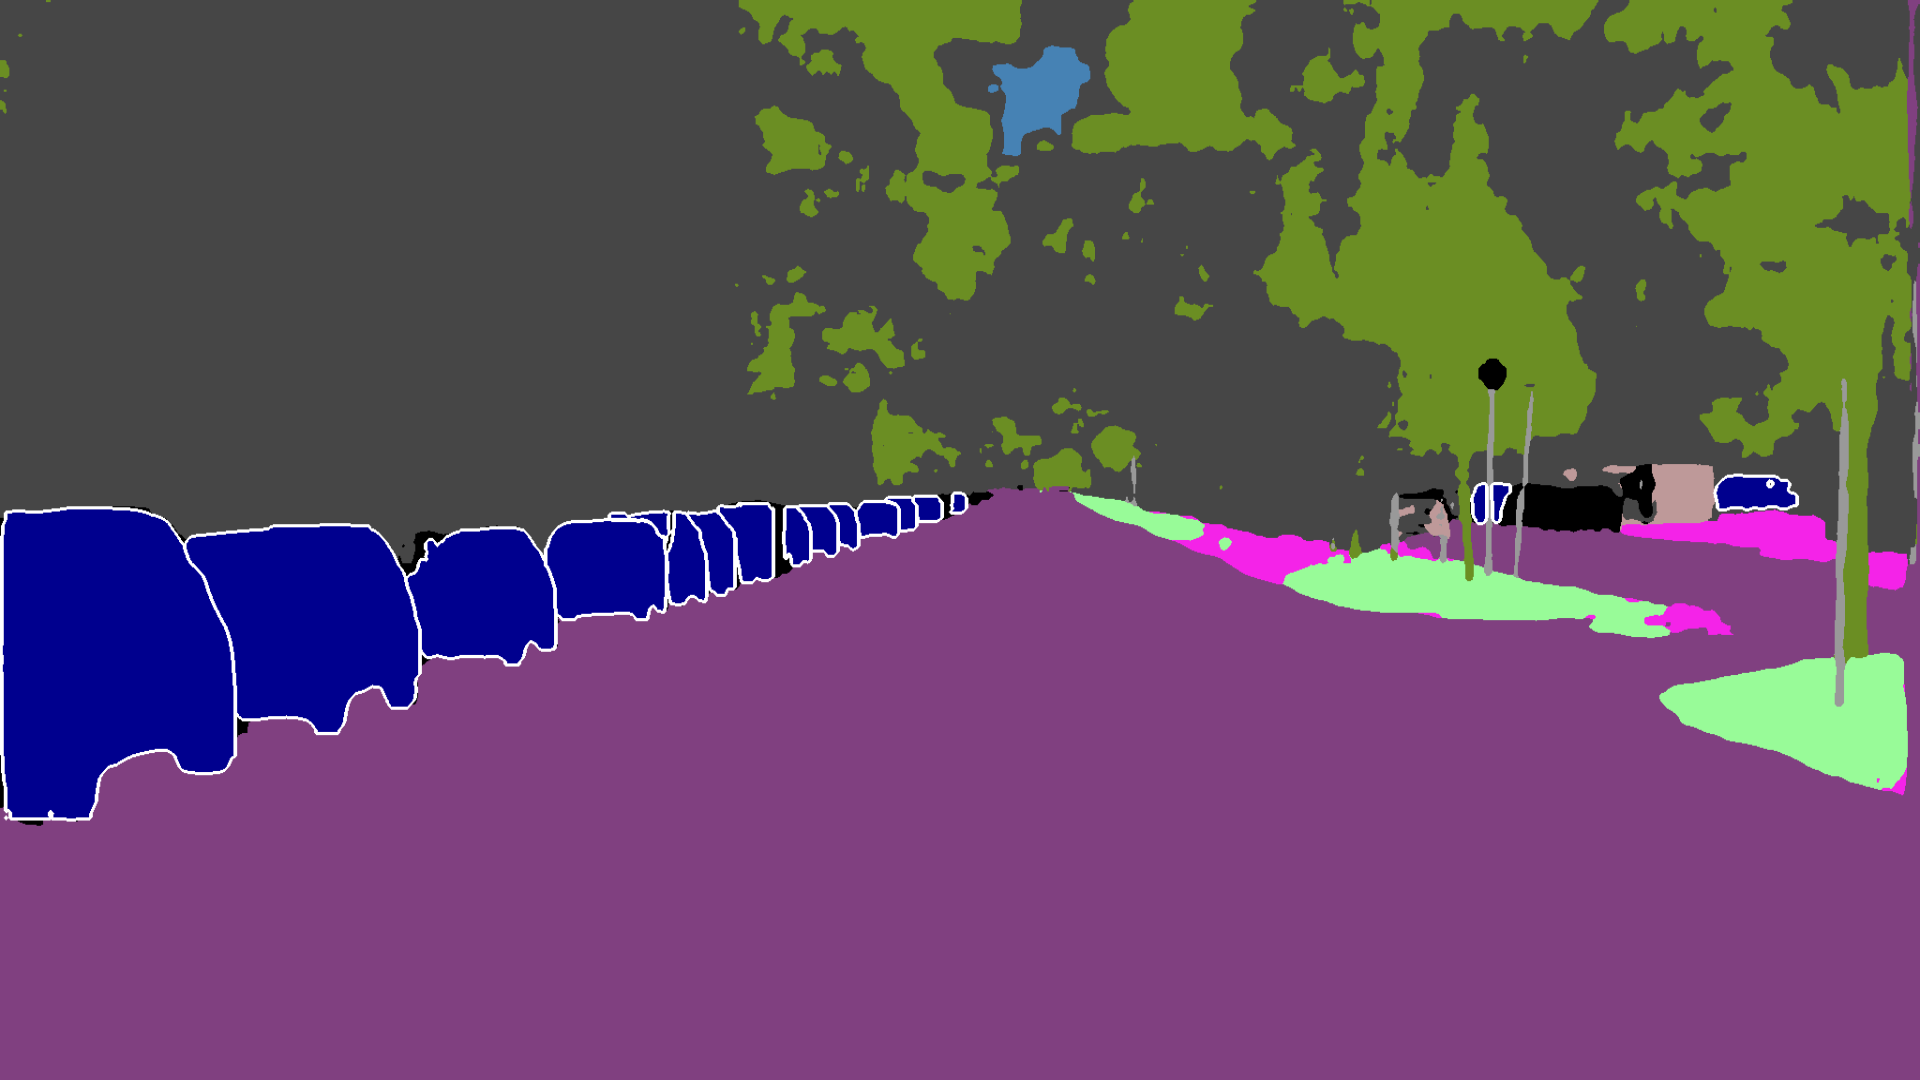
\includegraphics[width=0.6\textwidth]{figures/resultado_primario.png}
\legend{Fonte: Criação própria}
\label{fig:resultado_inicial}
\end{figure}

\begin{figure}[!ht]
\centering
\caption{Expectativa do resultado do EfficientPS.}
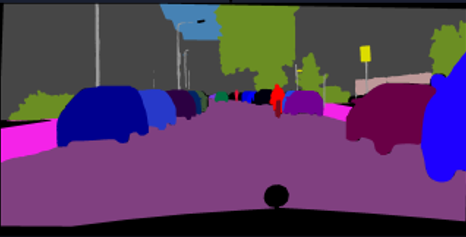
\includegraphics[width=0.6\textwidth]{figures/expectativa.png}
\legend{Fonte: \citeonline{mohan2020efficientps}}
\label{fig:expectativa}
\end{figure}

Seguindo os passos citados em uma publicação de \citeonline{efficientps_issue23} no repositório de \citeonline{efficientpsGit}, o resultado obtido não foi satisfatório, pois não foi possível discernir a que classes os segmentos pertenciam. O resultado é ilustrado na \cref{fig:resultado_obtido}.

\begin{figure}[!ht]
\centering
\caption{Resultado do EfficientPS obtido seguindo os passos da publicação no repositório.}
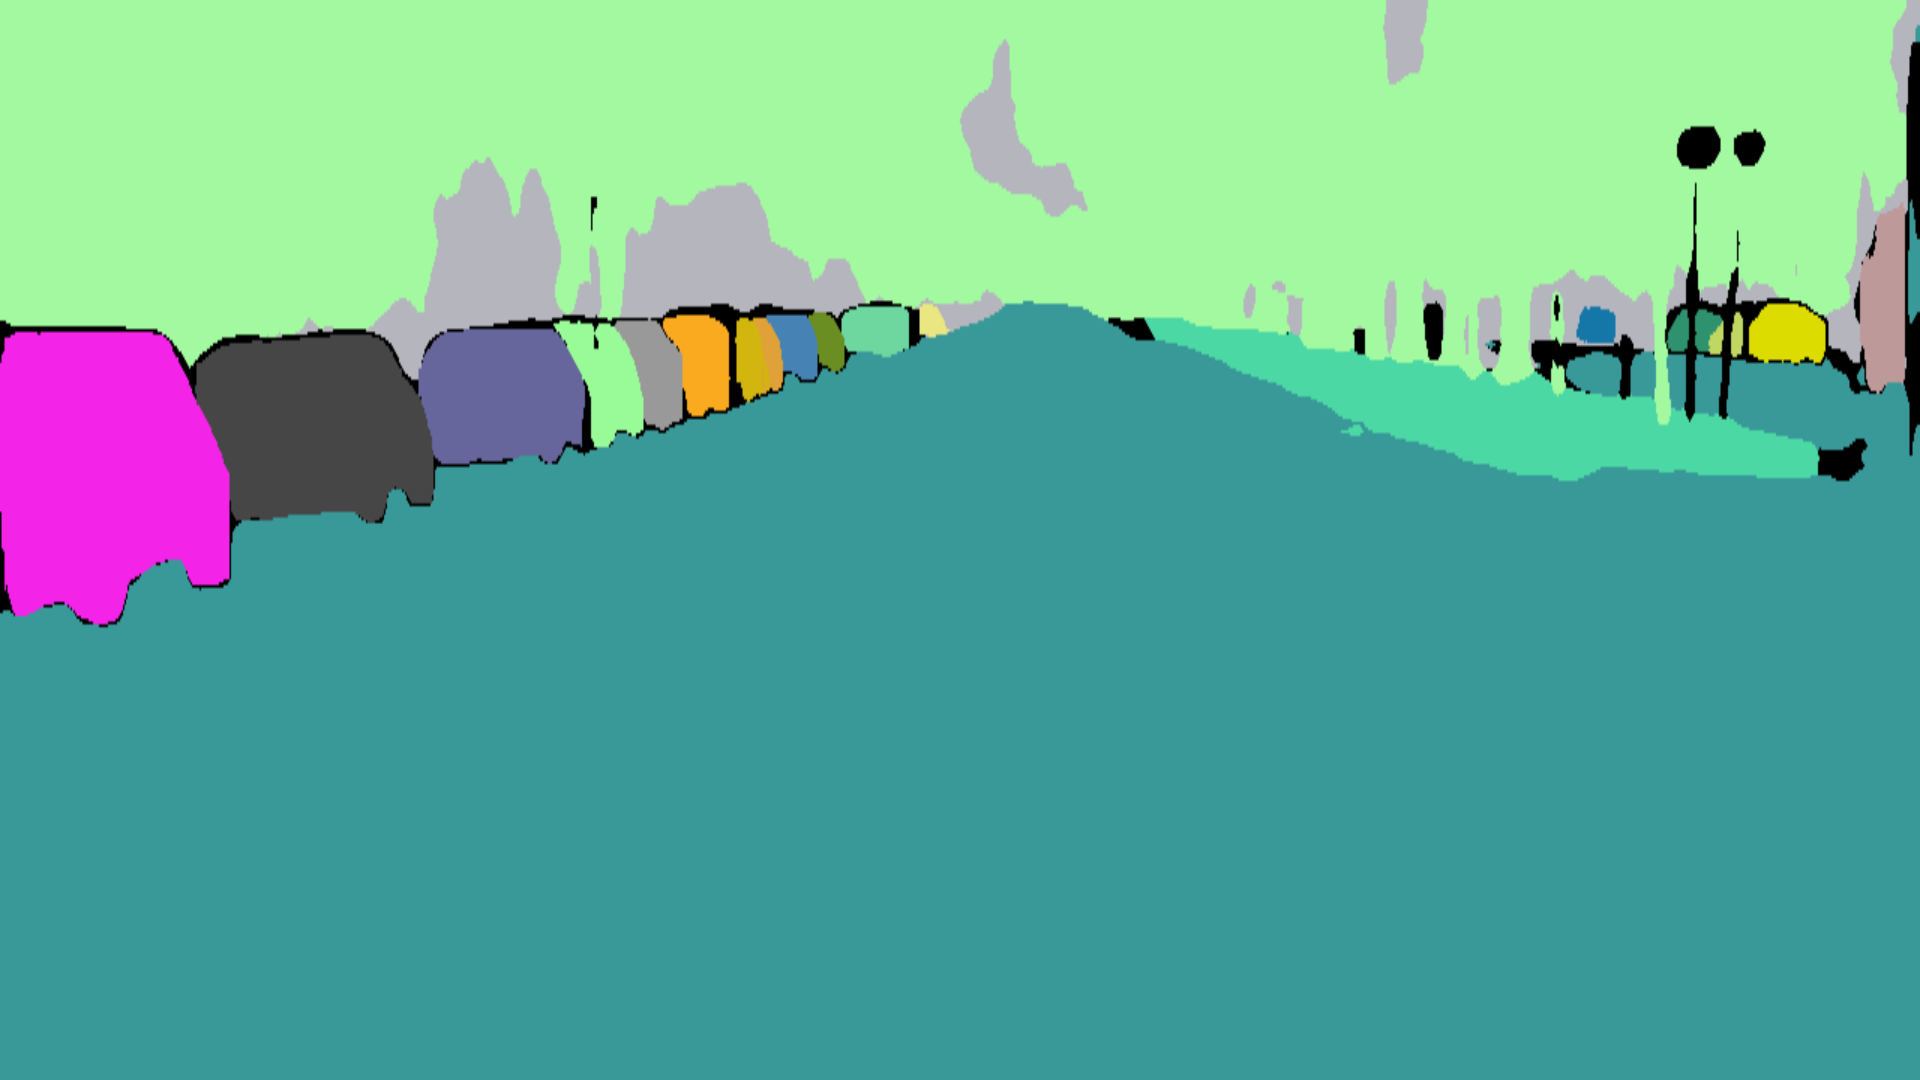
\includegraphics[width=0.6\textwidth]{figures/resultado_obtido.png}
\legend{Fonte: Criação própria}
\label{fig:resultado_obtido}
\end{figure}

\subsection{Selecionar contorno}

Para representar a seleção do contorno, utilizou-se uma técnica conhecida como imagem binária, que, segundo \citeonline{Embarcados}, consiste em isolar um objeto da imagem. Esta técnica pode ser usada como uma máscara para auxiliar no processamento do mapa no contorno desejado \cite{Aznag2020}.

Foram empregadas duas abordagens para selecionar o contorno: seleção por cor e seleção por preenchimento de inundação. A seleção por cor, conforme descrito por \citeonline{OpenCVInRange}, isola tudo na imagem que corresponde a uma determinada cor. Já a seleção por preenchimento de inundação, segundo \citeonline{OpenCVFloodFill}, baseia-se em um algoritmo de expansão que compara com uma faixa delimitada de cores. Ambos resultam em uma imagem binária, que também pode ser utilizada para selecionar a foto com desenho diretamente.

\subsubsection*{Tratamento da imagem binária}

Existem duas formas de tratar a imagem binária.

A primeira, não utilizada devido à distorção que causa, ocorre após a saída dos algoritmos de seleção. O objeto selecionado é detectado, centralizado em uma nova imagem, recortado e redimensionado a partir do centro para formar uma imagem quadrada. Todos os passos são observáveis na \cref{fig:saidas_selecao} \cite{Embarcados}.

\begin{figure}[!ht]
\centering
\caption{Passos da seleção da saída da inteligência artificial.}
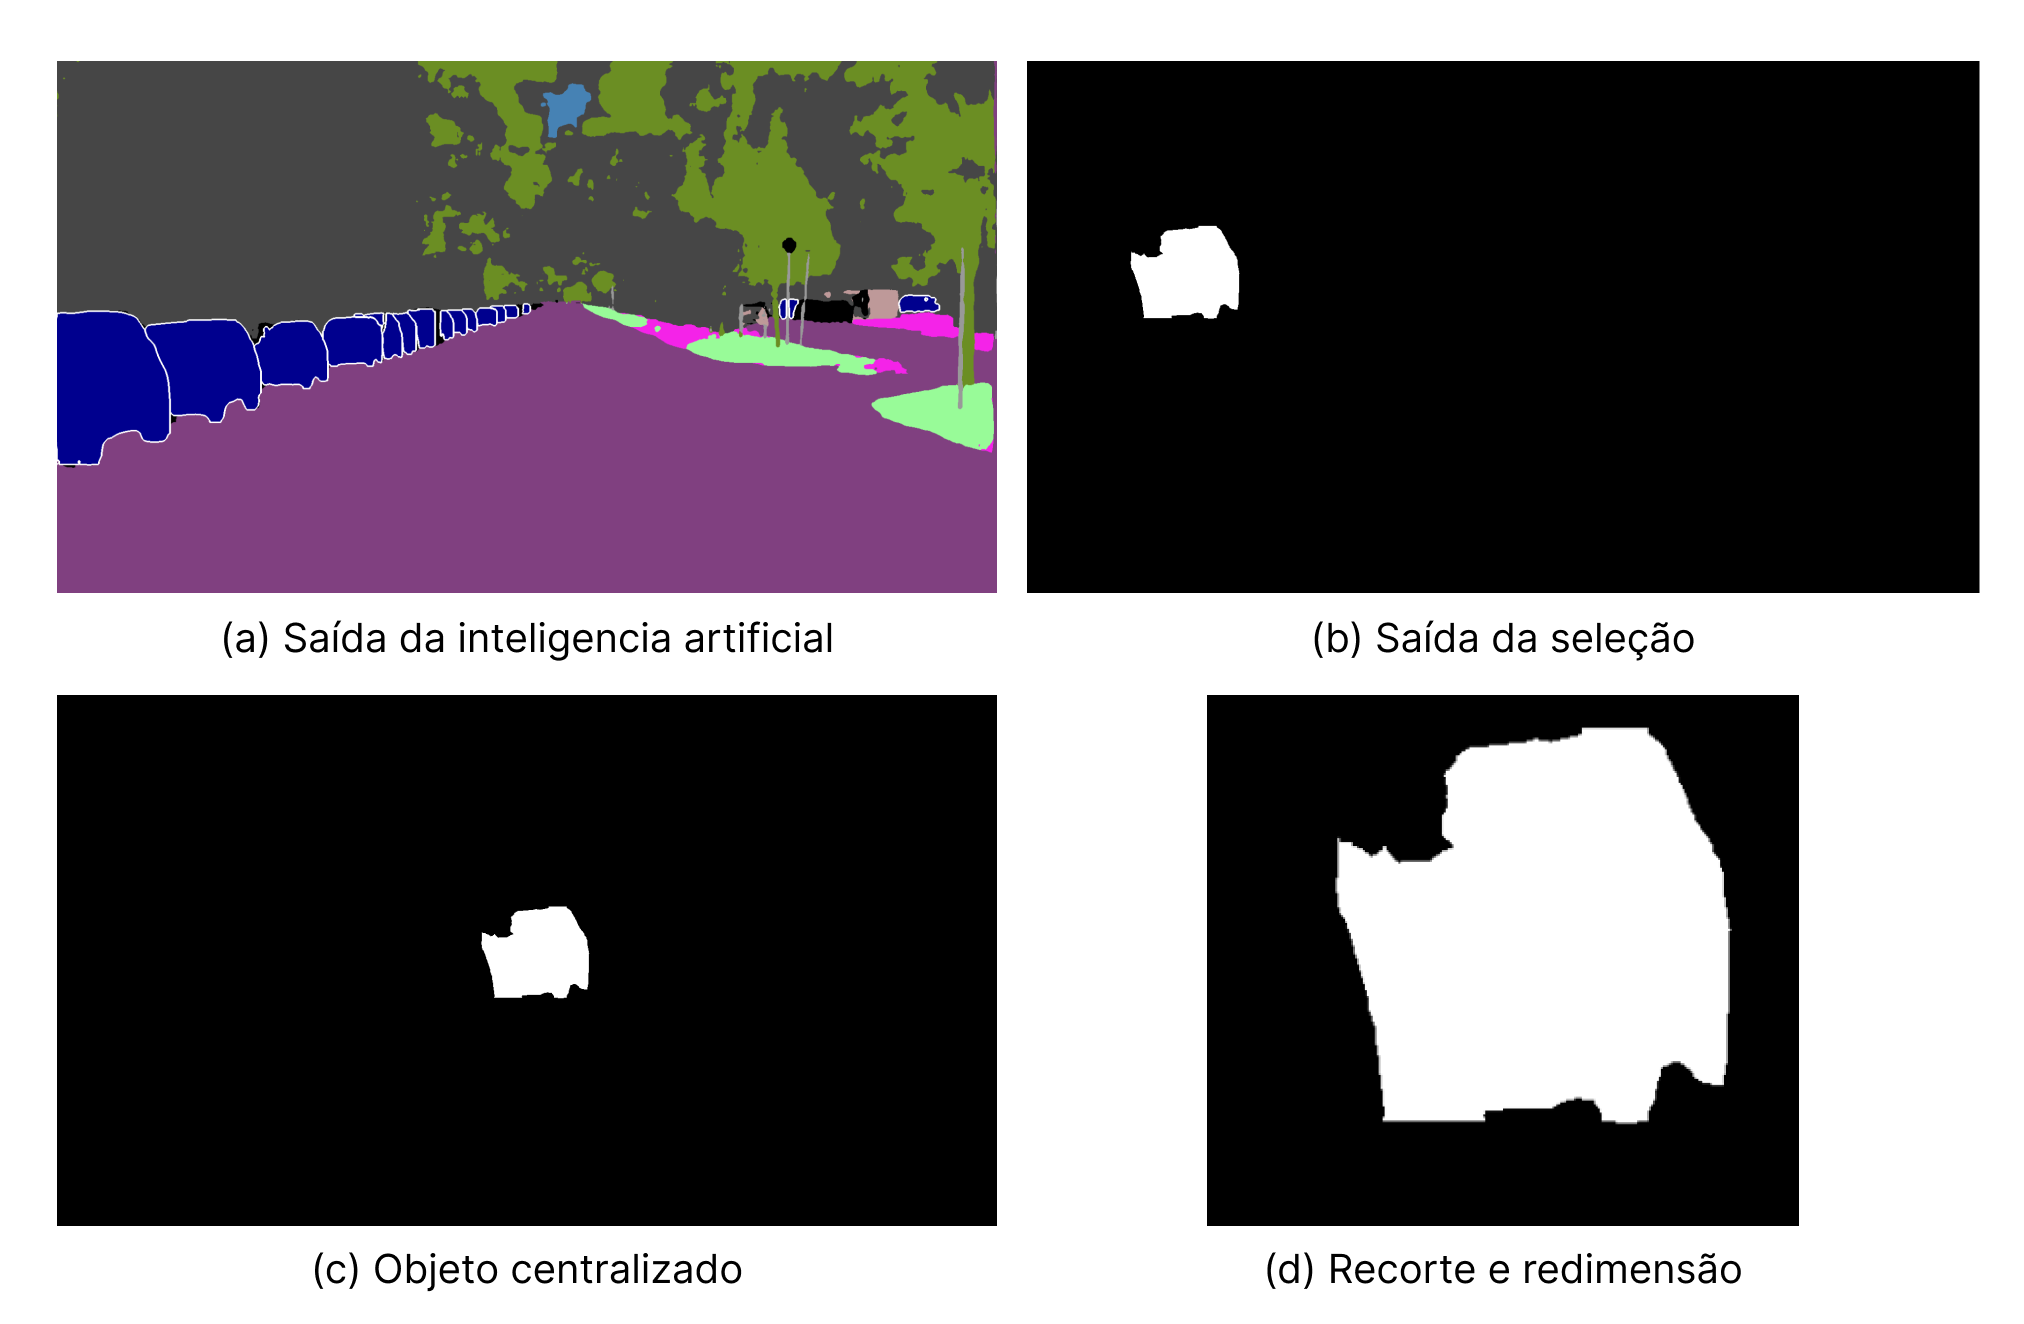
\includegraphics[width=1.0\textwidth]{figures/saidas_selecao.png}
\legend{Fonte: Autoria própria}
\label{fig:saidas_selecao}
\end{figure}

Já a segunda, mais eficiente, melhora os resultados evitando a distorção e a presença de bordas inadequadas. Este método localiza o objeto na imagem binária e recorta a imagem com as coordenadas e dimensões fornecidas. Em seguida, acrescenta-se uma borda na altura ou largura, conforme a folga entre as duas, transformando a imagem em quadrada. Após o redimensionamento para manter um padrão, adiciona-se novamente uma borda para representar o mar. Na \cref{fig:saidas_selecao_perf}, observa-se que o objeto não foi distorcido como no método anterior e permaneceu centralizado na imagem final \cite{Embarcados}.

\begin{figure}[!ht]
\centering
\caption{Passos da seleção da saída da inteligência artificial mais performática.}
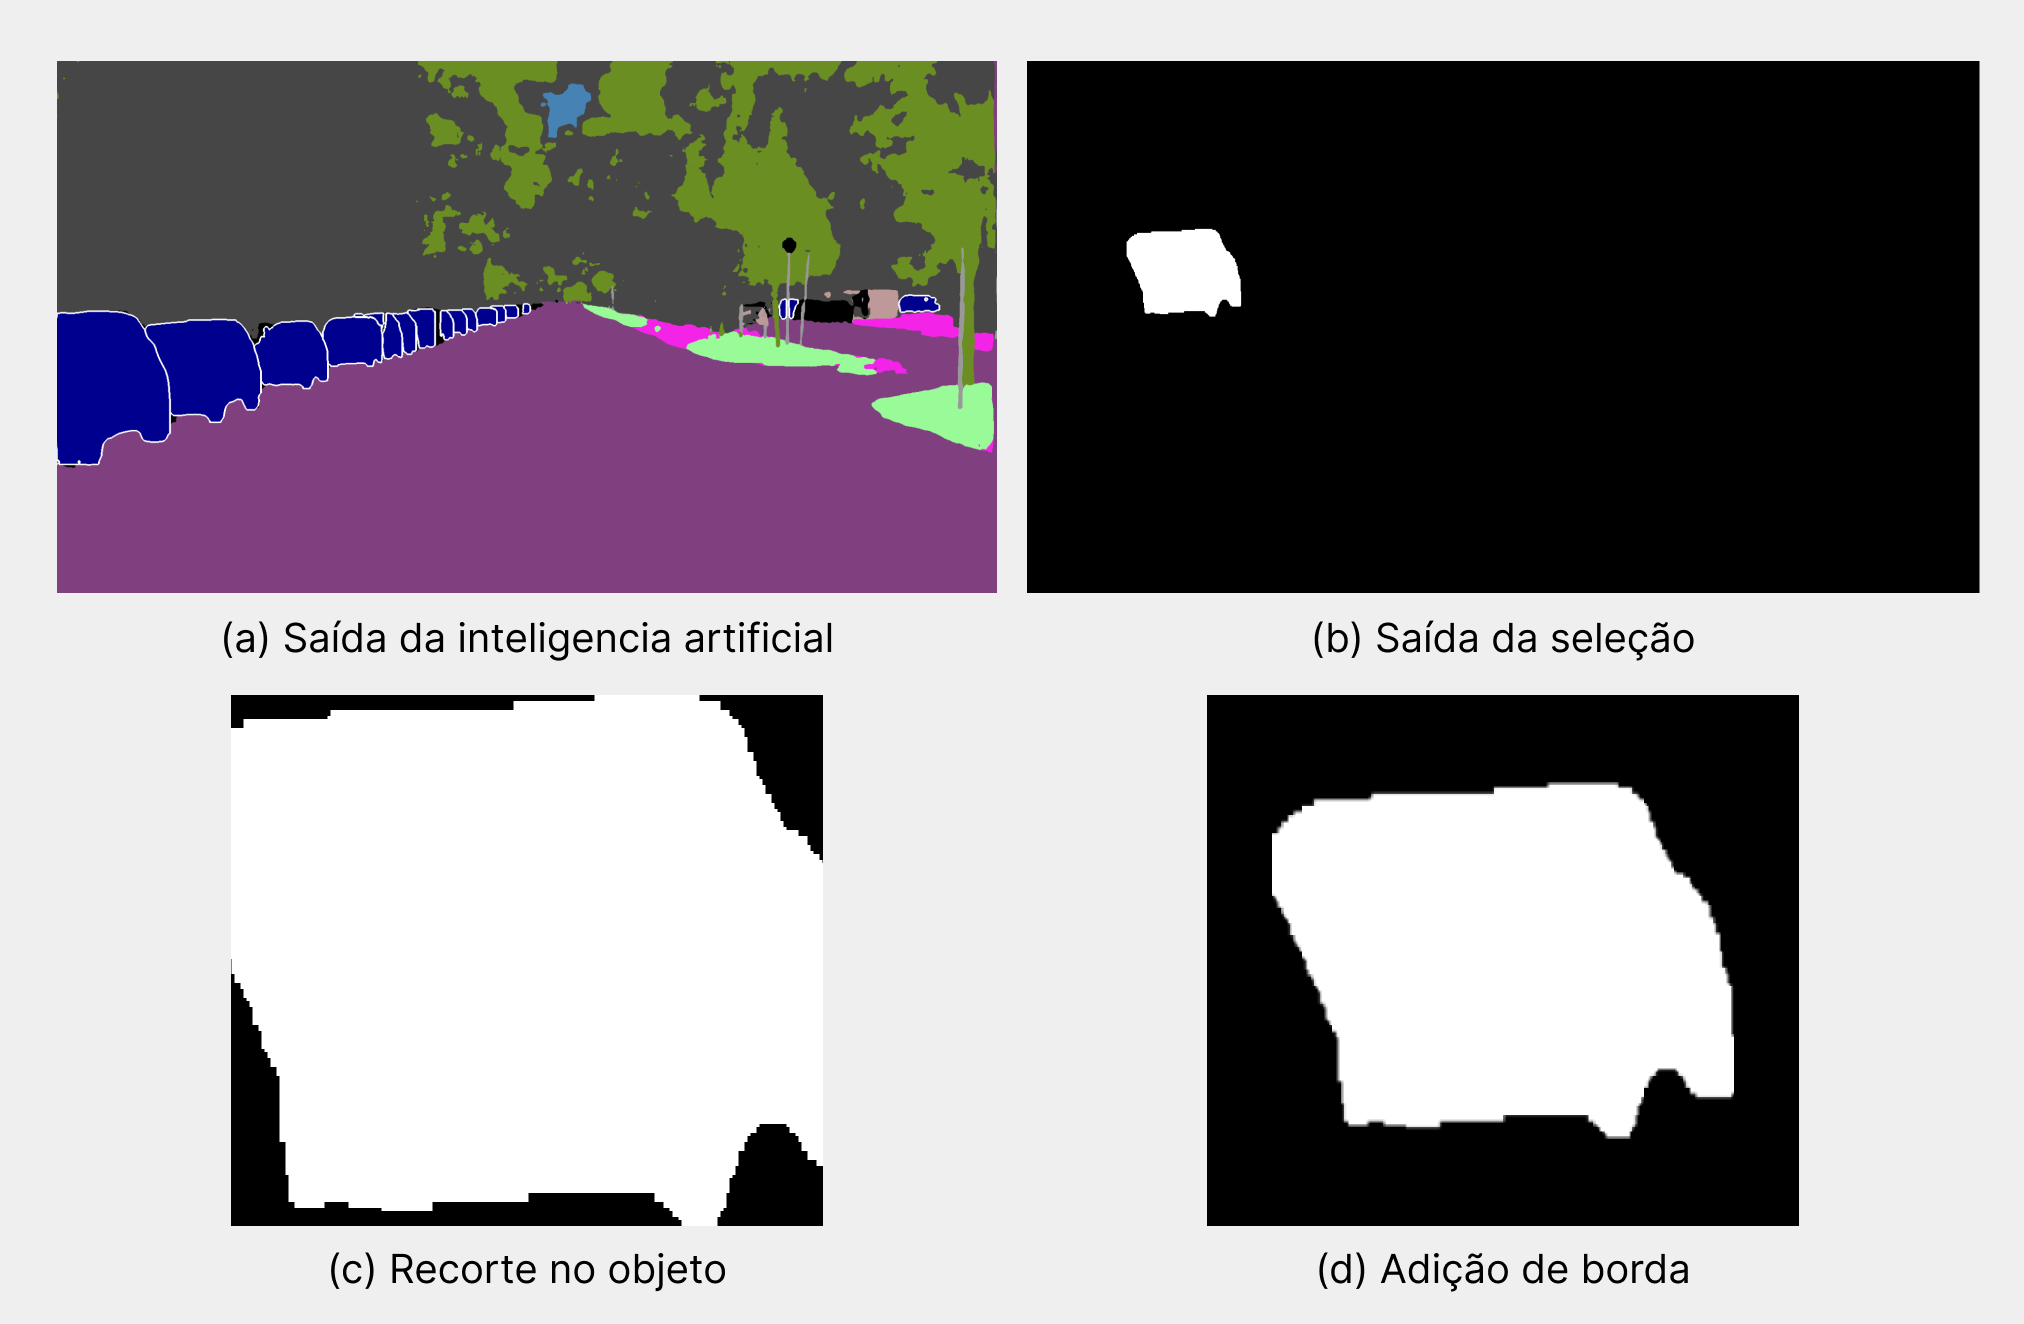
\includegraphics[width=1.0\textwidth]{figures/saidas_selecao_2.png}
\legend{Fonte: Autoria própria}
\label{fig:saidas_selecao_perf}
\end{figure}

\subsection{Geração procedural do mapa}

A base para a geração procedural do mapa foi o artigo de \citeonline{amitp2010}, com uma implementação em Python realizada por \citeonline{polygonal-map-generation}.

\subsubsection{Ilha gerada no contorno}

Para gerar o mapa da ilha, é necessário criar um diagrama de Voronoi. Primeiro, define-se pontos de quantidade pré-estabelecida e localização pseudoaleatória, que serão os centroides dos polígonos. Os vértices dos polígonos são gerados a partir da intersecção entre retas perpendiculares aos pontos médios entre nós vizinhos. Esses nós vizinhos são encontrados por meio de uma circunferência no ponto, e, se existir algum ponto, ele é marcado como vizinho, definindo essa área como região, conforme descrito na \cref{eq:voronoi_regiao}. Em seguida, cria-se outro grafo com esses pontos. A definição dos vértices é ilustrada na \cref{fig:explicacao_vertice}, onde os pontos vermelhos são os centroides, ligados por linhas pretas para gerar pontos médios (amarelos), traçando uma reta perpendicular. A intersecção é representada pelo ponto azul, que se torna o vértice, e a cor rosa representa a aresta do polígono \cite{amitp2010,rodrigues_diagrama_2019}.

\begin{figure}[!ht]
\centering
\caption{Ilustração do processo de criação do polígono.}
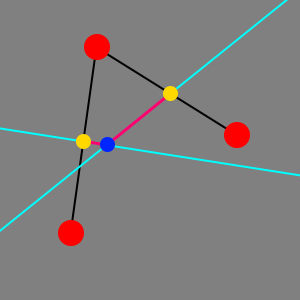
\includegraphics[width=0.6\textwidth]{figures/explicacao_vertice.png}
\legend{Fonte: Autoria própria}
\label{fig:explicacao_vertice}
\end{figure}

A \cref{fig:diagrama_voronoi_pontos} mostra o modelo do diagrama de Voronoi do algoritmo, onde os pontos vermelhos são os centroides, ligados por linhas pretas. Os pontos azuis são os vértices, conectados por linhas brancas para formar as arestas do polígono.

\begin{figure}[!ht]
\centering
\caption{Ilustração do diagrama de Voronoi.}
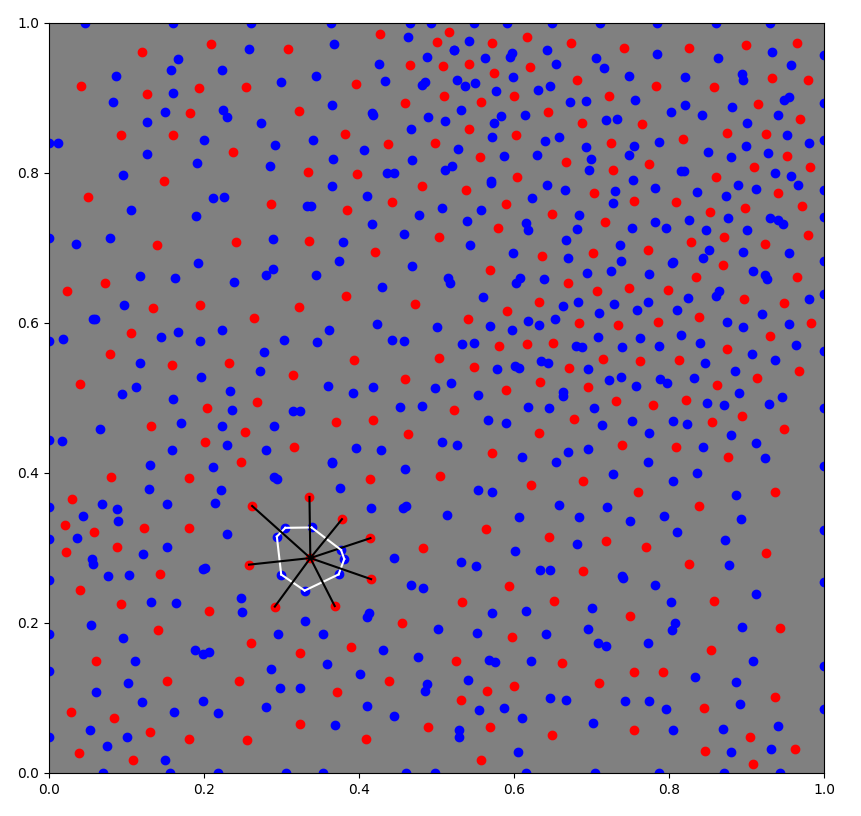
\includegraphics[width=0.6\textwidth]{figures/diagrama_voronoi_pontos.png}
\legend{Fonte: Autoria própria}
\label{fig:diagrama_voronoi_pontos}
\end{figure}

Cada polígono criado é denominado região, e basta definir o tipo do terreno, elevação e umidade. Na lógica, todos os polígonos com o terreno do tipo oceano são marcados. Há duas formas de selecionar o contorno da imagem.

A primeira, mais lenta, pois necessita verificar todos os pixels da imagem, percorre todos os pontos da imagem de entrada e verifica se cada pixel contido no objeto da imagem binária encontra-se nos polígonos gerados. Se encontrado, o polígono é adicionado a uma lista de marcação \cite{OpenCV}.

A segunda, mais performática, utiliza as bibliotecas do OpenCV. Faz-se uma iteração na lista de polígonos e, para cada um, cria-se uma imagem na qual o polígono da iteração é desenhado. Realiza-se uma comparação com a imagem binária, e o resultado dessa comparação é uma imagem com os pixels presentes em ambas as imagens (binária e do polígono). Verifica-se a existência de pixels brancos na imagem resultante e, se houver, adiciona-se o polígono à lista de marcação \cite{OpenCV}.

Para os polígonos na lista de marcação, marca-se o tipo do terreno como terra. Em seguida, verifica-se quais polígonos do tipo terra são vizinhos do tipo oceano. Se forem, define-se como do tipo litoral, e também se marcam os pontos desses polígonos que se encontram no polígono do tipo oceano \cite{amitp2010,Embarcados}.

Para calcular a elevação dos polígonos, inicialmente calcula-se a elevação das arestas de todos os polígonos. Isso é feito a partir de uma busca em profundidade que começa em todas as arestas tocando a borda do gráfico. A cada nova iteração, as arestas que tocam os cantos recebem o valor 0, e a altura evolui à medida que se aproxima do centro do mapa. Depois, realiza-se o cálculo de redistribuição de elevação. Com base na elevação calculada anteriormente, forma-se uma lista ordenada pela elevação, da menor para a maior. Cada item da lista é enumerado com um índice i e, com essa enumeração, calcula-se usando a \cref{eq:total_indexes}. Em seguida, calcula-se a \cref{eq:vertex_elevation}, sendo X a elevação do vértice. Finalmente, para calcular a elevação do polígono, faz-se a média dos vértices que pertencem ao polígono \cite{amitp2010}.

\begin{equation}
	\label{eq:total_indexes}
	Y = i / total de indices
\end{equation}

\begin{equation}
	\label{eq:vertex_elevation}
	X = sqrt(fator) - sqrt(sqrt * (1 - Y))
\end{equation}

Para a criação dos rios, busca-se os vértices do tipo terra e litoral que possuem uma elevação mínima definida, ou se os vértices se localizam próximos de um lago; então, armazena-se em uma lista. Seleciona-se, de forma pseudoaleatória, uma quantidade de vértices e verifica-se o tipo de terreno dos vizinhos dos vértices e das arestas que foram tocadas pelos vértices. Para cada um desses, é verificado se o tipo de terreno é terra ou litoral. Após isso, busca-se em todas as arestas a dona do vértice; ao encontrar, é marcado como sendo um rio \cite{amitp2010}.

Na geração de umidade, atribui-se um valor para cada vértice que possui uma aresta do tipo rio, ou se é vizinho de um lago, e coloca-se esse item em uma fila. Logo em seguida, busca-se, em profundidade, em todos os vértices adjacentes dos itens da fila, e calcula-se uma nova umidade a partir de uma multiplicação de um fator com o valor da umidade anteriormente atribuída. Verifica-se se os vértices adjacentes possuem uma umidade maior que a nova umidade calculada; se possuírem, coloca-se o vértice adjacente na fila e atribui-se o valor da nova umidade. Para terrenos do tipo oceano, é atribuído o valor máximo de umidade \cite{amitp2010}.

Por fim, atribui-se o valor da umidade para os polígonos e redistribui-se a umidade a partir de uma lista de polígonos com umidades ordenadas. Para cada item \textit{i}, executa-se a \cref{eq:umidade} e, assim, calcula-se o valor final da umidade \cite{amitp2010}.

\begin{equation}
\label{eq:umidade}
i / tamanho(lista) - 1
\end{equation}

Para assinalar os biomas, verifica-se o tipo do terreno, altura e a umidade; cada um desses parâmetros liga-se a um determinado bioma. E, para a atribuição final, aplica-se a classificação descrita na \cref{fig:diagrama-whittaker}. Porém, editou-se o eixo de temperatura para elevação, para chegar nos resultados da \cref{tab:biomes}, pois o diagrama de Whittaker não leva em consideração a elevação \cite{amitp2010}.

\begin{sidewaystable}
	\centering
	\caption{Relação entre umidade e elevação para biomas}
	\label{tab:biomes}
	\begin{tabularx}{\textwidth}{|X|X|X|X|X|X|X|}
	\hline
	\textbf{Zona de Elevação} & \multicolumn{6}{c|}{\textbf{Zona de Umidade}} \\
	\cline{2-7}
	 & \textbf{6 (úmido)} & \textbf{5} & \textbf{4} & \textbf{3} & \textbf{2} & \textbf{1 (seco)} \\
	\hline
	\textbf{4 (alto)} & \multicolumn{3}{|c|}{NEVE} & TUNDRA & DESNUDO & ESCALDADO  \\
	\hline
	\textbf{3} & \multicolumn{2}{|c|}{TAIGA} & \multicolumn{2}{|c|}{ARBUSTIVO} & \multicolumn{2}{|c|}{DESERTO TEMPERADO} \\
	\hline
	\textbf{2} & FLORESTA TROPICAL TEMPERADA & \multicolumn{2}{|c|}{FLORESTA DECÍDUA TEMPERADA} & \multicolumn{2}{|c|}{GRAMADO} & DESERTO TEMPERADO  \\
	\hline
	\textbf{1 (baixo)} &  \multicolumn{2}{|c|}{FLORESTA CHUVOSA TROPICAL} & \multicolumn{2}{|c|}{FLORESTA SAZONAL TROPICAL} & GRAMADO & DESERTO SUBTROPICAL  \\
	\hline
	\end{tabularx}
\end{sidewaystable}

Para gerar o mapa tridimensional, é gerada uma imagem denominada "mapa de altura", construída com base nos dados de elevações do grafo. Gera-se uma imagem com tonalidades de cinza, sendo que o pixel branco, com valor 255, representa o ponto mais alto do mapa, e o pixel preto, com valor 0, representa o ponto mais baixo. Isso é possível observar na \cref{fig:heightmap} \cite{planetzoo}.

\begin{figure}[!ht]
	\centering
    \caption{Exemplo de mapa de altura.}
	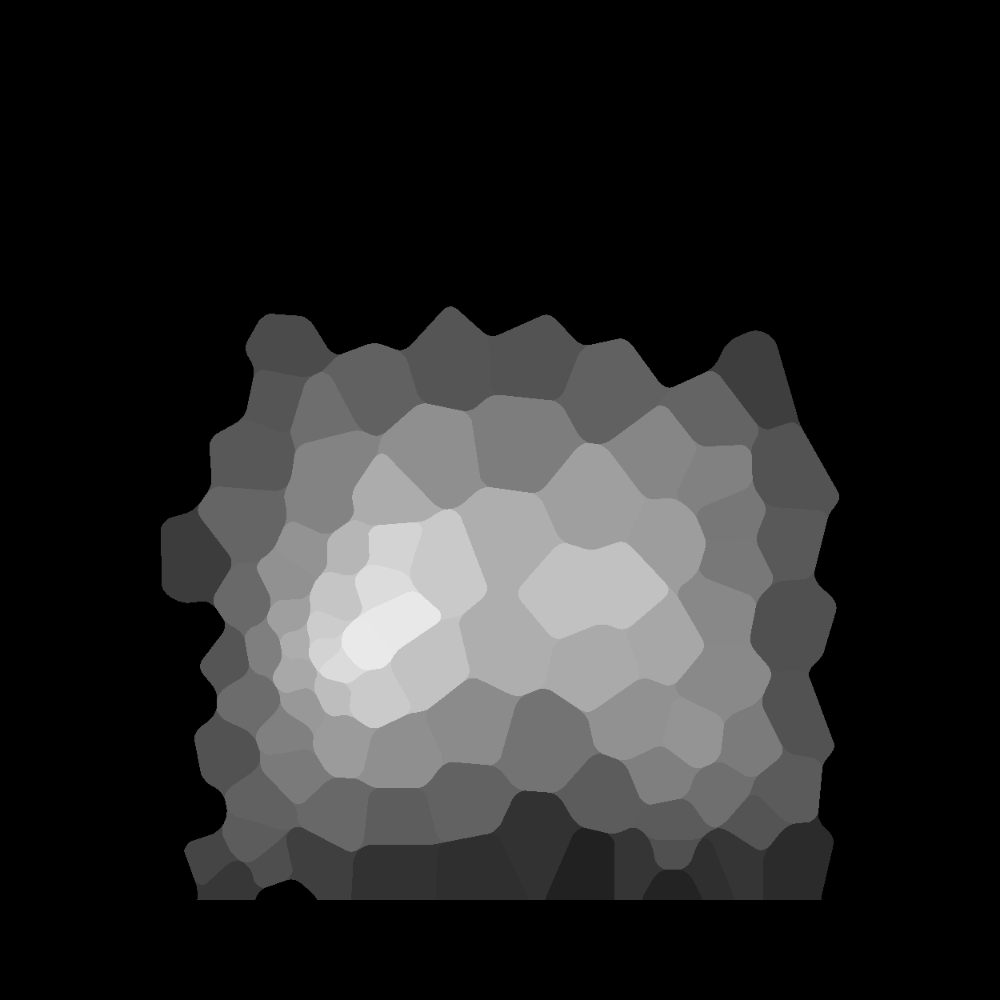
\includegraphics[width=0.6\textwidth]{figures/heightmap_eample.png}
    \legend{Fonte: \space Autoria própria}
	\label{fig:heightmap}
\end{figure}

\subsubsection{Unity - Mapa 3D}

Para demonstrar uma aplicação das imagens, utilizou-se o motor gráfico Unity. Criou-se uma automatização entre a geração do mapa e a atualização no projeto Unity. Este processo pode ser dividido em três partes: o terreno, o minimapa em 3D e a jogabilidade \cite{unitywebpage}.

\subsubsubsection{Terreno}
Para atualizar o terreno, utilizou-se primeiramente o pacote \textit{Terrain Tools}, que facilita o processo, pois é possível usar um mapa de altura em PNG ou RAW para criar um terreno. Ao executar, cria-se um terreno no qual o pixel mais branco (255) corresponde à altura mais alta \cite{unity-terrain-tools}.

Porém, esse processo era manual, e a ideia era que fosse automatizado. Logo, utilizou-se um algoritmo ligado à câmera do personagem que, ao iniciar a cena, atualiza o terreno com a nova imagem de mapa 3D em RAW. O algoritmo abre a imagem e percorre-a, anotando o relevo proporcionalmente a uma matriz, e depois aplica no terreno \cite{unity-terrain-tools}.

Além da funcionalidade de relevo, adicionou-se um pacote para alterar a textura de acordo com a altura, a fim de diferenciar o oceano da ilha e o bioma de floresta. Utilizou-se o pacote denominado \textit{Terrain Toolkit 2017}. No script, carregam-se as texturas e definem-se alguns parâmetros para atualizar com o terreno \cite{unity-terrain-toolkit}.

\subsubsubsection{Minimapa}
A saída da geração procedural visa dois principais resultados: o mapa de altura para definir o terreno e o mapa 2D que pode ser usado como minimapa \cite{unitywebpage}.

Para usar o mapa 2D como minimapa de forma automatizada, foi necessário adicionar nos \textit{scripts} uma conversão de uma imagem em formato PNG para um Sprite (2D e UI), atualizando as propriedades do objeto de jogo. Isso possibilita a localização de um ícone representando o jogador nesse minimapa, por meio da projeção das coordenadas 3D do mundo do jogo em um mapa 2D \cite{unitywebpage}.

\subsubsubsection{Jogabilidade}

Criou-se um personagem com movimentação para andar pelo mapa, baseado no vídeo do YouTube de \citeonline{firstPersonMovement}. Adicionando os objetos e o script principal, além de criar uma tag de chão para detectar a colisão, é possível jogar no mapa, andando em todas as direções e pulando.

\subsection{Testes}

Criaram-se testes para comparar uma combinação de imagens, que podem conter a imagem de entrada do algoritmo de geração procedural ou alguma de suas saídas, como mapa de altura ou mapa 2D. Para mensurar a qualidade, utilizou-se como base a técnica descrita por \citeonline{kirillov2019panoptic}, chamada de classificação dos conjuntos. Esta técnica cria uma nova imagem na qual cada pixel pertence a um conjunto dentre quatro: Verdadeiros Positivos, Verdadeiros Negativos, Falsos Positivos e Falsos Negativos. A \cref{fig:representacao} apresenta a ilustração da classificação dos conjuntos. A imagem a é a imagem de entrada para geração procedural (saída da seleção); a imagem b, o mapa de altura, é uma das saídas da geração procedural; a imagem c representa o filtro binário a partir do mapa de altura, ou seja, apenas os pixels com cor monocromática zero são mantidos como preto, e qualquer alteração é marcada como branco; a imagem d ilustra os conjuntos entre a imagem de entrada e o filtro binário do mapa de altura, sendo a cor cinza a união entre cores pretas, a cor branca a união de cores brancas, a cor verde quando a imagem de entrada tem cor branca mas o filtro binário tem cor preta e, por fim, a cor vermelha indica que o filtro tem a cor branca, mas na imagem de entrada tem a cor preta.

\begin{figure}[!ht]
	\centering
    \caption{Ilustração da classificação de conjuntos}
	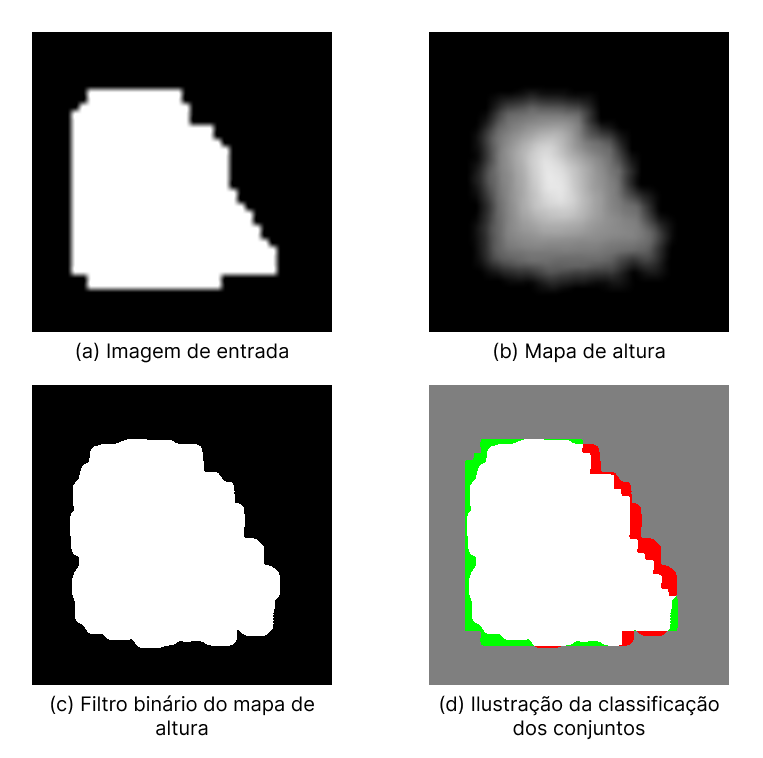
\includegraphics[width=0.8\textwidth]{figures/representacao_classificacao.png}
    \legend{Fonte: Autoria própria}
	\label{fig:representacao}
\end{figure}

Posteriormente, contabilizaram-se esses pixels com cores diferentes para utilizá-los em diversas métricas baseadas na classificação dos conjuntos, tais como: F1 Score, Coeficiente de Correlação de Matthews, Taxa de Descoberta Falsa, Taxa de Falso Negativo, Acurácia e União sobre Interseção \cite{Chicco2020, confusion_matrix_calculator, iou_metric_link}.

Além dessas métricas, empregou-se também uma métrica para o desfoque encontrado em uma imagem. Aplica-se um filtro para detectar bordas em x e y, calcula-se o gradiente e resulta-se no desvio padrão, o que serve para mensurar a harmonia do mapa de alturas. Outra métrica utilizada nos testes foi a duração do tempo no código, medida em segundos e contabilizando apenas a parte de geração procedural dos mapas.

Criou-se um teste genérico para ser reutilizado em diversos testes e facilitar a reprodução em caso de mudanças. Na chamada do teste, define-se as imagens e as métricas, possibilitando definir todas as combinações possíveis. Para cada combinação, serão executadas cinco imagens de entrada pré-definidas. Em cada imagem, percorrer-se-á um laço baseado em alguma variável de geração procedural, como tamanho do filtro de desfoque, quantidade de pontos ou tamanho da borda no mapa 2D. Em cada iteração da variável, o processo será repetido três vezes.

Em cada iteração de todos esses laços aninhados, será gerado proceduralmente algum mapa ou ambos, processadas as métricas e armazenados os resultados. Após isso, calcular-se-á a média das métricas e criada uma tabela em \LaTeX como resultado.

\subsection{Pós-processamento}
Analisando o resultado gerado no Unity do mapa 3D na \cref{fig:Unity_init}, percebe-se que não existe harmonia entre os biomas. Portanto, gerou-se uma solução aplicando um desfoque na imagem do mapa de altura para suavizar a mudança de biomas.

\begin{figure}[!ht]
	\centering
    \caption{Resultado no Unity sem usar filtro de desfoque no mapa de altura.}
	\includegraphics[width=0.8\textwidth]{figures/Unity_entry.png}
    \legend{Fonte: Autoria própria}
	\label{fig:Unity_init}
\end{figure}

Aplicando um filtro — ou kernel — de desfoque de tamanho 100x100, obteve-se o resultado ilustrado na \cref{fig:Unity_blur}. No entanto, ao analisar a \cref{tab:blur_error_input_output_3d}, observa-se que as métricas pioraram. Isso indica que o desfoque comprometeu a qualidade da equivalência dos contornos, exacerbando um problema de escala. Este problema é evidenciado pelo fato de que apenas o erro no mapa de altura foi detectado. Na \cref{fig:comparando_blur}, observa-se uma representação visual da classificação dos conjuntos definida em \citeonline{kirillov2019panoptic}, sendo a imagem a o resultado da comparação entre a imagem de entrada e a saída do mapa de altura sem desfoque, com o vermelho indicando o erro encontrado no mapa de altura (está branco no mapa de altura, mas preto na entrada), e a imagem b, o mesmo caso, porém aplicando o filtro de desfoque.

\begin{figure}[!ht]
	\centering
    \caption{Resultado no Unity usando filtro de desfoque no mapa de altura.}
	\includegraphics[width=0.8\textwidth]{figures/Unity_blur.png}
    \legend{Fonte: Autoria própria}
	\label{fig:Unity_blur}
\end{figure}

\begin{table}[h]
            \centering
            \caption{Resultados dos testes de contorno}
            \label{tab:resultados-contorno}
            \begin{tabular}{|c|c|c|}
                \hline
                                Tamanho filtro & IoU & Blur \\
                \hline
                0 & 0.7385 & 53.49246\\
        100 & 0.60484 & 9.75581\\
                \hline
            \end{tabular}
        \end{table}




\begin{figure}[!ht]
	\centering
    \caption{Ilustração da classificação de conjuntos entre a imagem de entrada e o mapa de altura}
	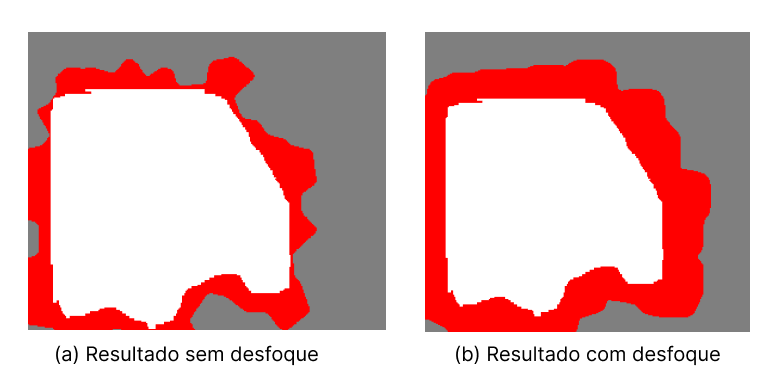
\includegraphics[width=0.8\textwidth]{figures/comparacao_blur.png}
    \legend{Fonte: Autoria própria}
	\label{fig:comparando_blur}
\end{figure}

Para tratar esse problema, adotou-se uma solução baseada em redimensionar a imagem e adicionar uma borda, diminuindo assim o tamanho do mapa de altura. Redimensionou-se uma imagem de 1000x1000 para 800x800, reduzindo-a em 20\%, e depois adicionou-se uma borda de cor preta em todos os lados de tamanho 100, retornando ao tamanho original. Para encontrar o melhor tamanho do filtro de desfoque nessas condições, executaram-se testes alterando o tamanho do filtro após a aplicação da técnica de redução do mapa. Os resultados estão na \cref{tab:blur_solution_input_output_3d}. Para selecionar o melhor resultado, definiu-se o critério de ter a menor métrica de desfoque — significando mais desfoque na imagem — e uma variação máxima de 1\% na métrica IoU em comparação com a métrica sem o filtro de desfoque. Assim, selecionou-se o resultado com filtro de tamanho 80, pois a métrica IoU apresentou 79\%, semelhante ao tamanho de filtro 0. Percebeu-se também que a diminuição da borda resultou em uma maior correspondência entre os erros da imagem de entrada e do mapa de altura.

\begin{table}[h]
    \centering
    \caption{Resultados dos testes entre imagem de entrada e output3d}
    \label{tab:blur_solution_input_output_3d}
    \begin{tabular}{|c|c|c|c|c|}
        \hline
        Tamanho filtro & Desfoque & IoU & FDR & FNR \\
        \hline
        100 & 11.35778 & 0.76178 & 0.22752 & 0.01707\\
        90 & 11.88265 & 0.76887 & 0.2162 & 0.02281\\
        80 & 12.37601 & 0.79299 & 0.18761 & 0.02824\\
        70 & 13.59314 & 0.79101 & 0.18298 & 0.03676\\
        60 & 14.75522 & 0.80283 & 0.16196 & 0.04787\\
        50 & 16.29726 & 0.81851 & 0.13458 & 0.06073\\
        40 & 18.35148 & 0.81608 & 0.12325 & 0.07635\\
        30 & 21.52558 & 0.81866 & 0.10467 & 0.0935\\
        20 & 27.79682 & 0.8183 & 0.08627 & 0.11246\\
        10 & 38.13084 & 0.80744 & 0.07181 & 0.13757\\
        0 & 48.89338 & 0.79895 & 0.05978 & 0.15749\\
        \hline
    \end{tabular}
\end{table}




Após a melhoria do resultado do mapa de entrada, é necessário ajustar o mapa 2D, visto que este deve ser bastante semelhante ao mapa de altura, para informar, por exemplo, a localização exata do personagem no jogo, com visualização do mapa inteiro. Observa-se na \cref{tab:border_2d_solution_output_2d_output_3d} os resultados obtidos dos testes com o tamanho da borda adicionada ao mapa 2D, sendo que o maior valor de IoU obtido foi de 60%.

\begin{table}[h]
    \centering
    \caption{Resultados dos testes entre mapa 2d e mapa de altura}
    \label{tab:border_2d_solution_output_2d_output_3d}
    \begin{tabular}{|c|c|c|c|}
        \hline
        Tamanho borda & IoU & FDR & FNR \\
        \hline
        0 & 0.82075 & 0.02435 & 0.16192\\
        10 & 0.84148 & 0.02679 & 0.13833\\
        20 & 0.86438 & 0.03616 & 0.10622\\
        30 & 0.87938 & 0.04263 & 0.0846\\
        40 & 0.89456 & 0.05307 & 0.0578\\
        50 & 0.90031 & 0.06612 & 0.03827\\
        60 & 0.90771 & 0.07929 & 0.0152\\
        70 & 0.89229 & 0.10441 & 0.00408\\
        80 & 0.86867 & 0.13132 & 1e-05\\
        90 & 0.84037 & 0.15963 & 0.0\\
        100 & 0.81396 & 0.18604 & 0.0\\
        \hline
    \end{tabular}
\end{table}




\subsection{Interface Gráfica}

Utilizou-se a biblioteca PyQt5 para criar uma interface gráfica, na qual o usuário pode interagir e criar um mapa a partir da seleção do contorno detectado pelo modelo de IA.

Esse módulo é responsável por conectar todas as partes e obter o mapa. Portanto, é necessário abrir uma imagem do diretório local, carregar e disparar a execução do processo de segmentação de imagem. Após o resultado da IA, permite-se a seleção do contorno, cria-se uma imagem binária a partir do contorno e envia-se como argumento na geração procedural de mapas.

Além disso, para promover a usabilidade, utilizou-se um \textit{loading} específico para o PyQt5. Para isso, foi necessário usar threads, criando classes para executar as tarefas de forma separada e síncrona.